\subsection{Session 2, Exercise 3}

\lineparagraph{Exercise}

Let $\Sigma=\{0,1\}$. Give a deterministic finite automaton that accepts the words that contain at least three $1$'s.

\lineparagraph{Solution}


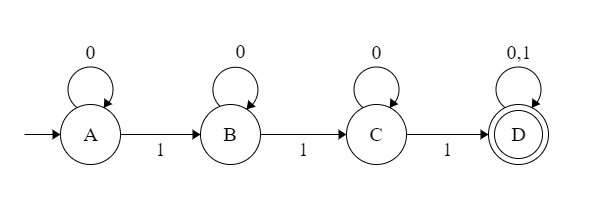
\includegraphics[width=0.6\linewidth]{02/2_3.png}

Proof:

Let's look at what the states mean:

\begin{itemize}
    \item A: State $A$ represents words that contain no $1$'s.
    \item B: State $B$ represents words that contain exactly one $1$.
    \item C: State $C$ represents words that contain exactly two  $1$'s.
    \item D: State $D$ represents words that contain at least three  $1$'s.
\end{itemize}

Let's look at the starting state and the accepting and rejecting states:

\begin{itemize}
    \item The starting state is the state that should represent the empty string. The empty string contains no $1$'s, which is represented by $A$, so the starting state is $A$.
    \item The only accepting state is $D$, since we want to accept words that contain at least three $1$'s, which is represented by state $D$.
    \item $A$,$B$ and $C$ are rejecting states, since they represent words that contain less than three $1$'s, which are not in the language.
\end{itemize}

Let's look at the transitions:

\begin{itemize}
    \item Transitions $A\xrightarrow{1}B$, $B\xrightarrow{1}C$, $C\xrightarrow{1}D$: the amount of $1$'s in the word is incremented by one, which means we should move one step closer to state $D$.
    \item Transitions $A\xrightarrow{0}A$, $B\xrightarrow{0}B$, $C\xrightarrow{0}C$: Reading in a $0$ does not change the current state. It does not move us closer to state $D$, however it does not ruin any progress already made, since the $1$'s don't have to be consecutive. So we just stay in the current state, discarding the incoming $0$'s.
    \item $D\xrightarrow{0,1}D$: when we have already seen at least three $1$'s, seeing characters ($0$'s or $1$'s) will not give us additional benefits, we can already accept the word as is, so we just stay in state $D$ until we reach the end of the input.
\end{itemize}